

%% Lee
%% In dissertation, change section* to chapter and subsection* to section


\chapter{System Overview}
\label{chap-five}
\label{sec:System Overview}
As mentioned in chapter \ref{sec:Introduction} and chapter \ref{Motivation}, this works target application processes mulltiple \acp{ann} each of which have limited opportunities for both weight reuse and batch processing.
These requirements require \ac{dram} to be employed for main storage of \ac{ann} parameters and local \ac{sram} is of limited use.
Under these conditions, the \ac{dram} bandwidth is the system bottleneck.

To meet these requirements, this work proposed employing \acp{3dic} technology along with a customized \ac{3d} \ac{dram} and \ac{asic} technology. 
By physically staying within the \ac{3dic} footprint and taking advantage of high density \acp{tsv} this work is able to maintain a significantly higher bandwidth over 2D or 2.5D \ac{asic} or \ac{asip} solutions.
The objective was to demonstrate that a pure \ac{3dic} system can implement multiple disparate \acp{ann} within reasonable power and area constraints. 

The \ac{3dic} system die stack (figure \ref{fig:3DICStack}) includes the \ac{3d}-\ac{dram} with a system manager below and one or more processing layers below the manager.
\begin{figure}[!t]
% the [] contains position info e.g. [!t] means here
\centering
\captionsetup{justification=centering}
\captionsetup{width=.9\linewidth}
\centerline{
\mbox{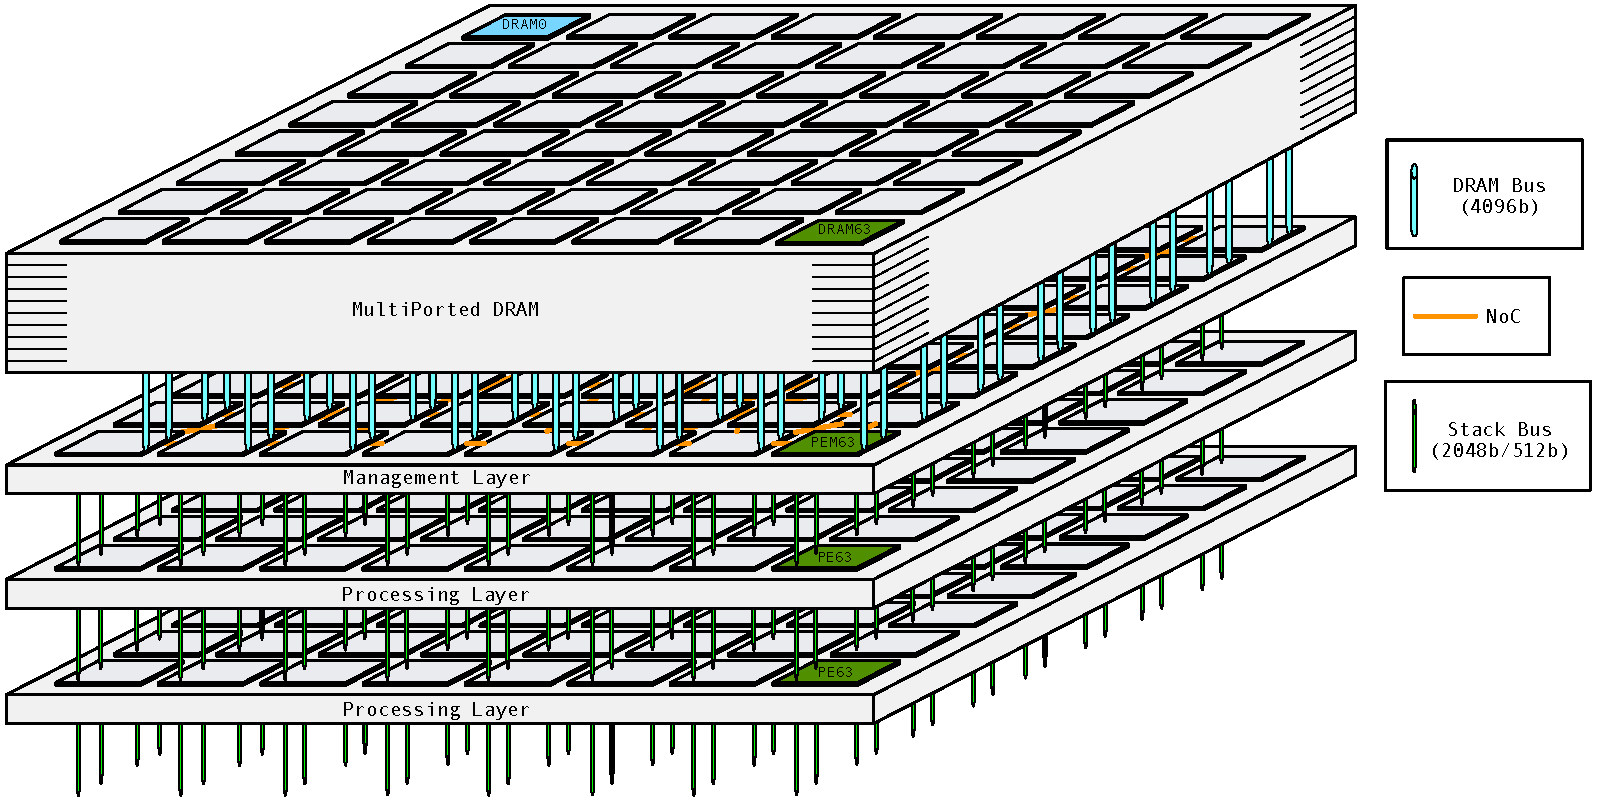
\includegraphics[width=.9\linewidth]{StackDiagram}}
}
\caption{3DIC System Stack}
\label{fig:3DICStack}
\end{figure}

3D-DRAM has recently become available in standards such as \ac{hbm} and \ac{hmc} and proprietary devices such as the DiRAM4 available from Tezzaron. 
These technologies provide high capacity within a small footprint.

In the case of \ac{hbm} and \ac{diram4} \cite{tezzaron:diram4}, the technology can be combined with additional custom layers to provide a system solution.

The question becomes, can a useful system coexist within the same 3D footprint?

This work targeted a baseline system with:
\begin{outline}
  \1 Computations requiring single precision floating point
  \1 Tezzaron \acf{diram4} \cite{tezzaron:diram4} for main memory
  \1 28nm \ac{asic} technology
\end{outline}
The work includes customizing the interface to a 3D-\ac{dram}, researching data structures to describe storage of \ac{ann} parameters, designing a memory manager with unique micro-coded instructions and a \ac{pe} layer.  
The targeted 3D-\ac{dram}, the Tezzaron DiRAM4 employs 64 disjoint memories arranged in a physical array.

This works system is designed such that a sub-system, known as a \acf{ssc} operates on one of the disjoint sub-memories within the \ac{diram4} (see figure \ref{fig:diram4Layout}).
As shown in figure \ref{fig:SSC}, the \ac{ssc} includes the \ac{diram4} sub-memory (referred to as the \ac{ssc} memory), a manager module and a \ac{pe} module.
The \ac{diram4} has 64 sub-memories so there are 64 \acp{ssc}. The \ac{ssc} has been designed as a standalone unit and does not have a knowledge of the other \acp{ssc} in the system.
\begin{figure}
\centering
\begin{subfigure}{.4\textwidth}
  \centering
  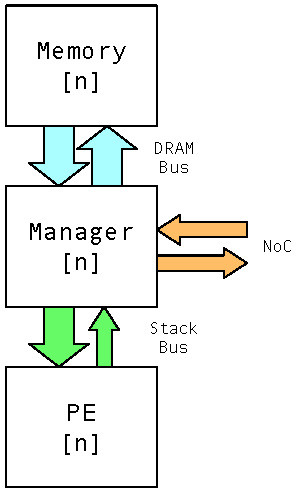
\includegraphics[scale=0.75]{SSC_logical}
  \captionsetup{justification=centering, skip=10pt}
  \vspace{-6pt}
  \caption{Sub-system column logical block diagram}
  \label{fig:Sub-system Column Logical Block Diagram}
\end{subfigure}%
\begin{subfigure}{.6\textwidth}
  \centering
  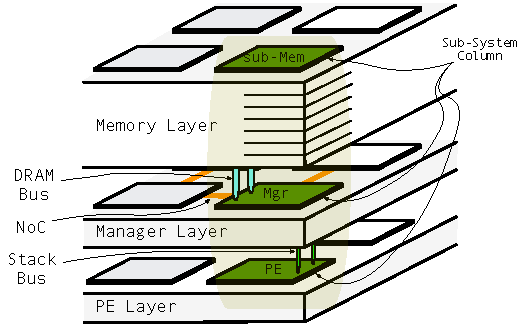
\includegraphics[scale=1.1]{SSC_physical}
  \captionsetup{justification=centering, skip=-27pt}
  %\vspace{36pt}
  \vspace{20pt}
  \caption{Sub-system column physical diagram}
  \label{fig:Sub-system Column Physical Diagram}
\end{subfigure}
\captionsetup{justification=centering, skip=12pt}
\caption{\acf{ssc}}
\label{fig:SSC}
\end{figure}

An overview of the various blocks and interconnects are given in sections \ref{sec:3ddram} through \ref{sec:Overview Summary}
with additional detail provided in chapter \ref{sec:Detailed System Description}.

% ----------------------------------------------------------------------------------------------------
\section{Customized \ac{dram} : \acf{diram4}}
\label{sec:3ddram}
The \ac{diram4} \cite{tezzaron:diram4} employs multiple memory array layers in conjunction with a control and IO layer.
The memory is formed from 64 disjoint sub-memories each providing upwards of \SI[per-mode=symbol]{1}{\giga\bit} with a total capacity of at least \SI[per-mode=symbol]{64}{\giga\bit}.
Unlike traditional \ac{dram}, the \ac{diram4} has two independent channel which are accessed using \ac{ddr} signalling on the control signals.
Each channel has 32 banks and 4096 pages per bank with \SI[per-mode=symbol]{4096}{\bit\per page}.

The standard \ac{diram4} has a 32-bit read databus and a 32-bit write databus enabling simultaneous read and write. Both read and write databuses employ \ac{ddr} signaling.
The read and write transactions are burst-of-two providing 64bits per read/write. When accessing a \ac{dram}, a read and write are often referred to as a cacheline.
The device is designed to operate at \SI[per-mode=symbol]{1}{\giga\hertz} although this work targeted a \SI[per-mode=symbol]{500}{\mega\hertz} clock frequency.

This work is proposing customizations to the \ac{diram4} which are outlined in chapter \ref{sec:DRAM Customizations}. One of these proposed changes is to widen the read and write databuses to 2048-bits.
Using the same burst-of-two means each read and write will access an entire page. A cacheline becomes 4096-bits.
Another proposed change is the add mask bits to the write databuse to avoid having to perform read/modify/writes when writing back data much smaller than the new large cacheline.

\begin{figure}[!t]
% the [] contains position info e.g. [!t] means here
\centering
\captionsetup{justification=centering}
\captionsetup{width=.9\linewidth}
\centerline{
\mbox{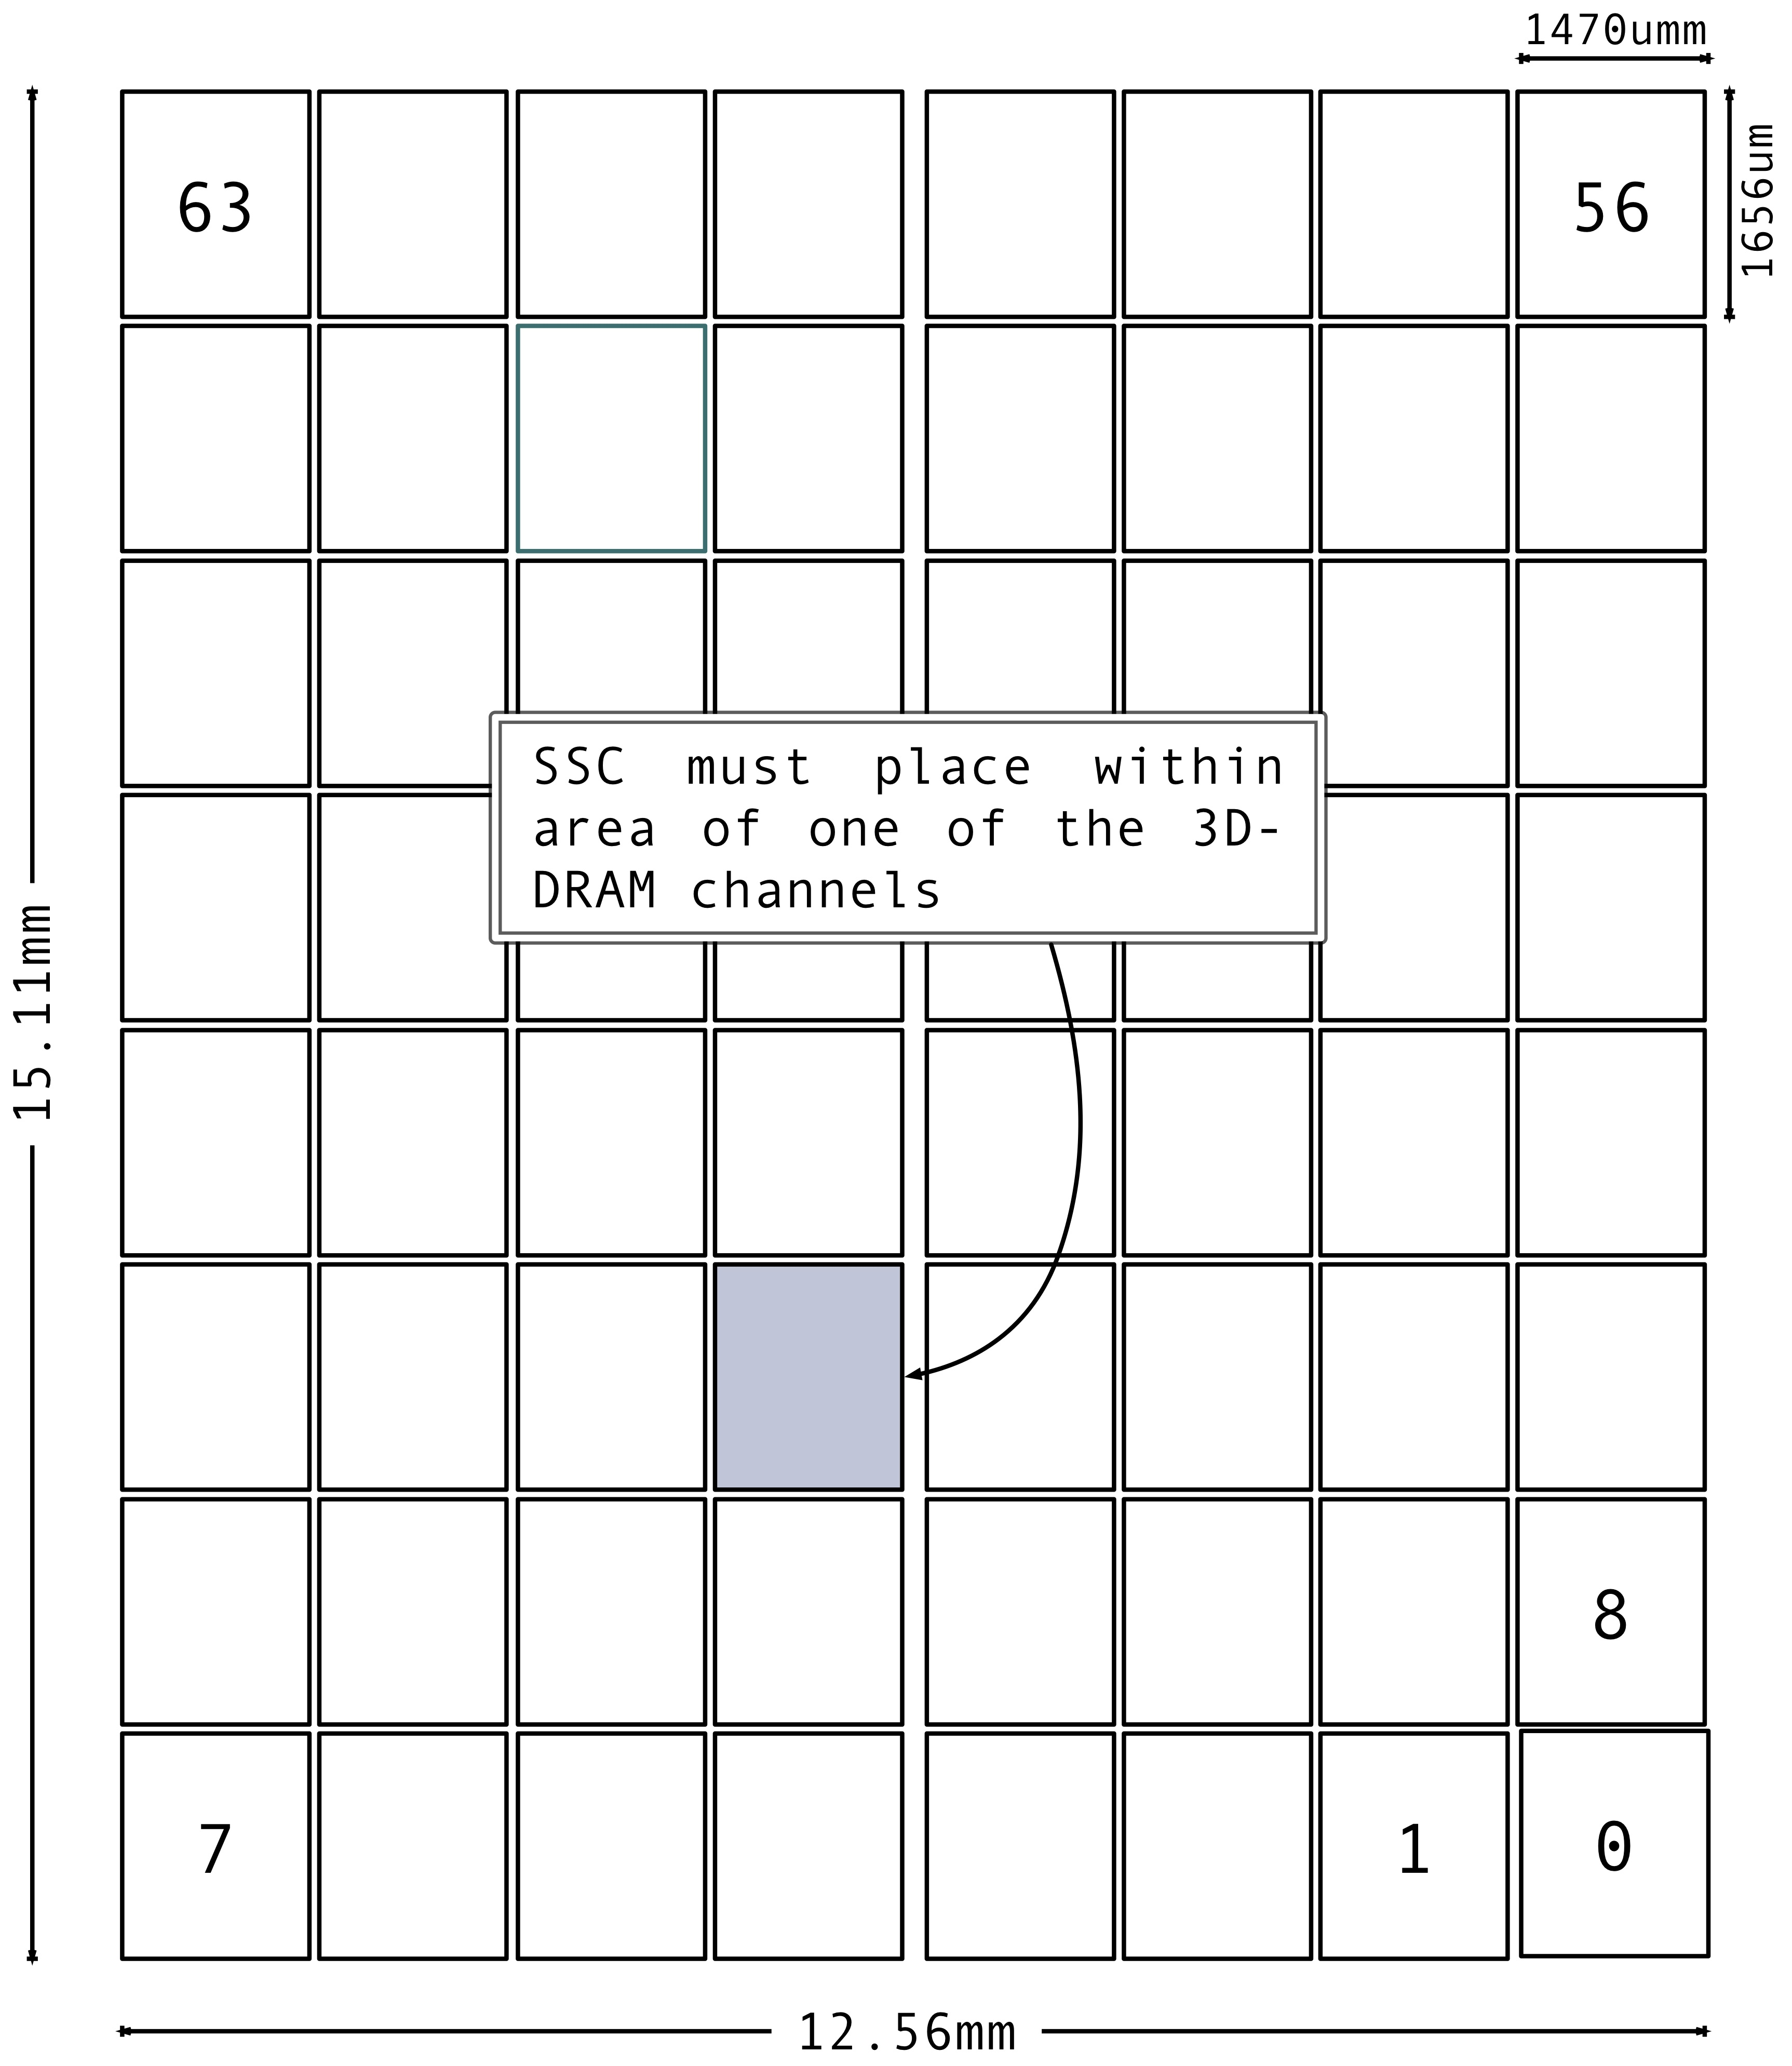
\includegraphics[width=.4\linewidth]{DiRAM4Layout}}
}
\caption{\ac{dram} Physical Interface Layout showing area for \ac{ssc}}
\label{fig:diram4Layout}
\end{figure}


% ----------------------------------------------------------------------------------------------------
\section{Manager Layer}
The Manager block is the main controller in the system. The operations required to process an \ac{ann} are formed from individual instructions which are decoded by the Manager. 
These instructions include descriptors to describe memory read operations, processing engine operations, memory write operations and general system operations for synchronization. 
The manager reads these system instructions from an instruction memory, decodes the instruction and configures the various blocks in the system.
The configuration includes:
\begin{itemize}
      \item initiate operand reads from \ac{dram}
      \item prepare the processing engine (\ac{pe}) to operate on the operands
      \item prepare the result processing engine to take the resulting \ac{an} activations from the \ac{pe} and write those results back to the \ac{dram}
      \item replicate the resulting \ac{an} activations to neighbor managers for processing of other \ac{ann} layers
\end{itemize}

% ----------------------------------------------------------------------------------------------------
\section{Processing Layer}
\label{sec:Processing Layer}
The \ac{pe} is able to operate on data streamed directly from the \ac{dram} via the Manager layer. 
The \ac{pe} is configured by the manager to perform operations on the operand data streamed from the manager. 
In the baseline system, the main operation is to perform multiply-accumulates on 32 execution lanes of two operands. 
These operands typically are the pre-synaptic \ac{an} activations and the connection weights. 
The \ac{pe} also performs the activation function on the result of the MAC to generate the \ac{an} activation value. 
These 32 activation values are sent back to the Manager layer.

% ----------------------------------------------------------------------------------------------------
\section{Layer Interconnect}
\label{sec:Layer Interconnect}

The layers are connected using through-silicon-vias (\ac{tsv}s) which provide high connection density, high bandwidth and low energy.
By ensuring the system stays within the 3D footprint ensures we can take advantage of the area and bandwidth benefits provided by \acp{tsv}.
The high density interconnect provided by \acp{tsv} allows the system to take advantage of the very wide \ac{dram} bus provided by the \ac{dram} customization described in section \ref{sec:Customization One: Very-Wide Bus}.
The wide interconnect between the manager and \ac{pe} are also implemented using \acp{tsv}.

The interconnect between the manager and \ac{pe} is referred to as the stack bus. The interconnect between the manager and \ac{dram} is referred to as the \ac{dram} bus.

% ----------------------------------------------------------------------------------------------------
\section{Inter-Manager Communication}
\label{sec:Inter-Manager Communication}

During configuration and/or computations, data must be transported between managers. 

During \ac{an} computations, the \ac{an} weights and states are read from the \ac{dram} in the \ac{ssc}.
This inter-manager communication is provided by an \ac{noc}.
When computing an \ac{ann} across multiple processing sub-systems, often \ac{an} activation data must be shared between these \ac{ssc}s. The \ac{ssc} includes the \ac{dram} port, the manager and the \ac{pe}. 
An \ac{noc} within each management block communicates with each adjacent manager using a mesh network. This \ac{noc} has a forwarding table that can be reconfigured to provide more efficient routing for a given processing step.

% ----------------------------------------------------------------------------------------------------
\section{Summary}
\label{sec:Overview Summary}

A control and data flow diagram of the stack showing the 64 sub-system columns can be seen in figure \ref{fig:FlowDiagram}.
\begin{figure}[!t]
% the [] contains position info e.g. [!t] means here
\centering
\captionsetup{justification=centering}
\centerline{
\mbox{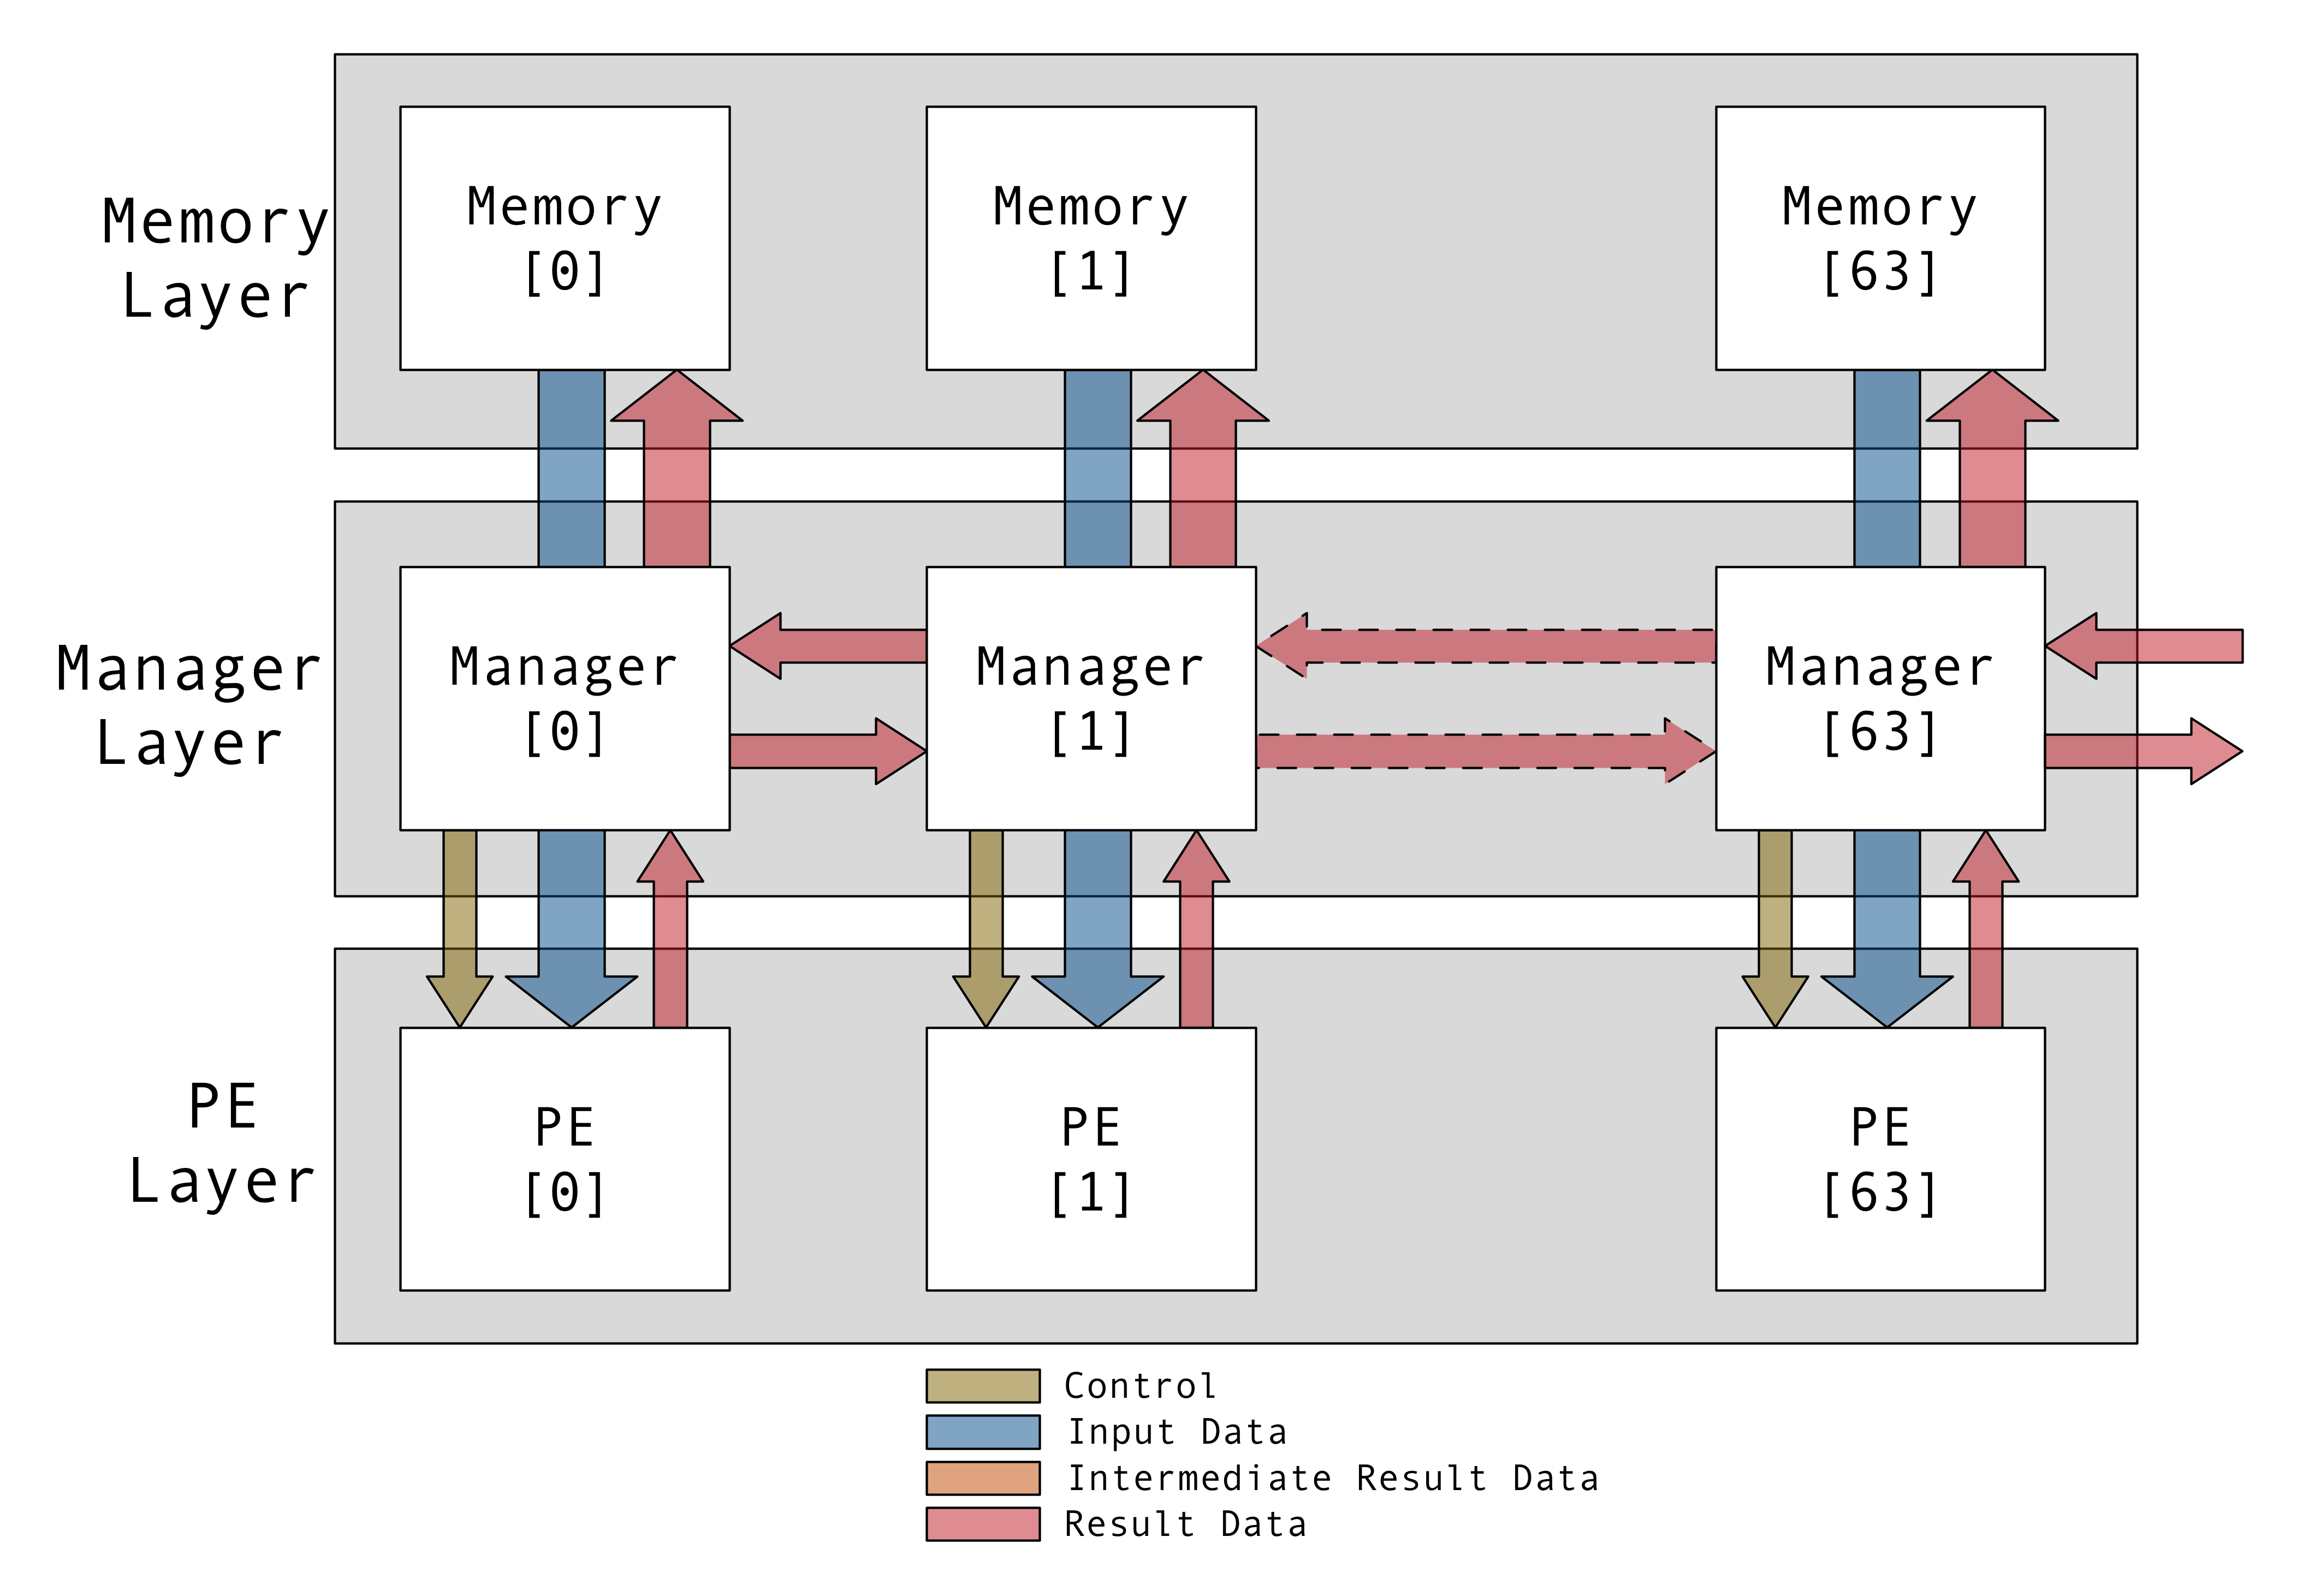
\includegraphics[width=.8\linewidth]{FlowDiagram.jpg}}
}
\caption{System Flow Diagram}
\label{fig:FlowDiagram}
\end{figure}

\subsection{Configuration, Command and Data Flow}
\label{sec:Configuration, Command and Data Flow}

All communication between \acp{ssc} is over an \ac{noc}. 
Some causes of communication between \acp{ssc} are host configuration, synchronization messages between \acp{ssc}, \ac{an} state replication etc..
\iffalse
Synchronization messages and \ac{an} state replication are a side effect of the instructions described in chapter \ref{sec:SystemOperations}.
\fi


